%\documentclass[a3paper]{article}
%\usepackage[left=0mm,top=1cm,right=0mm,bottom=0mm]{geometry}
\documentclass[border=0]{standalone}
\usepackage{tikz}
\usetikzlibrary{calc}
\usepackage{xcolor}
\definecolor{pGreen}{HTML}{006633}
\definecolor{pRed}{HTML}{cc0033}

\begin{document}
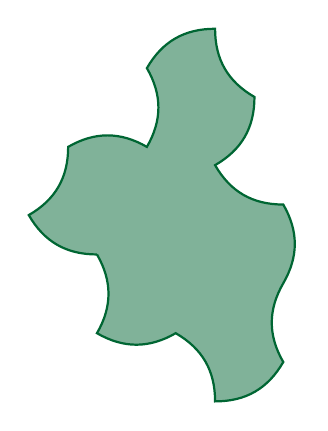
\begin{tikzpicture}
    \pgfmathsetmacro{\w}{1}	%scale
	\pgfmathsetmacro{\a}{1}
	\pgfmathsetmacro{\b}{1}

    \coordinate (A) at (0,0);
    \coordinate (A2) at ($(A) + (-90:\a*\w)$);
    \coordinate (A3) at ($(A2) + (0:\b*\w)$);
    \coordinate (A4) at ($(A3) + (-60:\b*\w)$);
    \coordinate (A5) at ($(A4) + (30:\a*\w)$);
    \coordinate (A6) at ($(A5) + (90:\a*\w)$);
    \coordinate (A7) at ($(A6) + (90:\a*\w)$);
    \coordinate (A8) at ($(A7) + (150:\a*\w)$);
    \coordinate (A9) at ($(A8) + (60:\b*\w)$);
    \coordinate (A10) at ($(A9) + (120:\b*\w)$);
    \coordinate (A11) at ($(A10) + (-150:\a*\w)$);
    \coordinate (A12) at ($(A11) + (-90:\a*\w)$);
    \coordinate (A13) at ($(A12) + (180:\b*\w)$);
    \coordinate (A14) at ($(A13) + (-120:\b*\w)$);

    \tikzset{
        monotile/.pic={
            \draw[draw=pGreen, thick,fill=pGreen!50] (A) to[bend left] (A2) to[bend right] (A3) to[bend left] (A4) to[bend right] (A5) to[bend left] (A6) to[bend right] (A7) to[bend left] (A8)to[bend right] (A9) to[bend left] (A10) to[bend right] (A11) to[bend left] (A12)to[bend right] (A13) to[bend left] (A14) to[bend right] (A);
        }
    };
	\draw (0,0) pic {monotile};
\end{tikzpicture}
\end{document}
